\chapter{Results}
% summary of the behavioral results per experiment
\section{Summary}
  We summarize the behaviors exhibited by the pigeon models in each experiment, categorized by their body speeds and the reward functions the controllers were trained with.

  \begin{itemize}
    \item Body speed 0; $r_{head\_stable\_manual\_reposition\_strict\_angle}$; $max\_offset = 0.5$
    \begin{description}
      \item The pigeon model managed to keep its head stationary as expected.
    \end{description}

    \item Body speed 1; $r_{head\_stable\_manual\_reposition\_strict\_angle}$; $max\_offset = 1.0$
    \begin{description}
      \item The pigeon model initially struggled to control its head in a specific pattern or position.
      However, after 5 seconds, it managed to align the head within the radius $max\_offset$ around the manually set position $T$, resulting in a generation of trajectory that depicts a pattern of thrust and hold phases.
      The final 5 seconds of the footage depicts the head and the limbs getting stuck on the topside of the body.
    \end{description}

    \item Body speed 1; $r_{head\_stable\_manual\_reposition}$; $max\_offset = 1.0$
    \begin{description}
      \item The pigeon model produced similar results to the previous experiment, with the exception of the overall performance.
      Due to the less strict definition of the reward function, it generated a trajectory that resulted in the acquirement of larger return, and as a result, a better performance in producing the desired head-bobbing behavior.
      In particular, the timespan of the head following the manually-defined trajectory was longer than those seen in the previous experiment.
    \end{description}

    \item Body speed 0; $r_{fifty\_fifty}$
    \begin{description}
      \item The head of the model moved around in the vicinity of a single position, similar to the baseline counterpart.
    \end{description}

    \item Body speed 1; $r_{fifty\_fifty}$
    \begin{description}
      \item The head of the model gradually leaned down and backwards as if it were following the surrounding stationary object.
    \end{description}

  \end{itemize}

\subsection{Learning Curves}
% LEARNING CURVES===!!!


% raw trajectories will NOT be included!

\section{Behavior Renderings}
% figures for behavior renderings explanation
  We rendered the resulting behaviors produced by controllers trained on aforementioned reward functions and environments into images or frames.
  Combining the frames generated for each of the 1000 timesteps and setting as 60 frames per second resulted in 33.35 second videos.
  The time-lapses presented in Figures \ref{fig:manual_trajectory_body_speed_0}, \ref{fig:manual_trajectory_strict_body_speed_1}, \ref{fig:manual_trajectory_not_strict_body_speed_1}, \ref{fig:fifty_fifty_body_speed_0}, and \ref{fig:fifty_fifty_body_speed_1} were created by sampling every $300$ frames within the last 30 seconds of the video.
  The frames' sequential order is from the top left to the bottom right.
  The camera is locked to follow the pigeon's body.
  % 60/5 * [10] = 300

% figures of pigeon behavior renderings
  \begin{figure}[H]
      \centering
      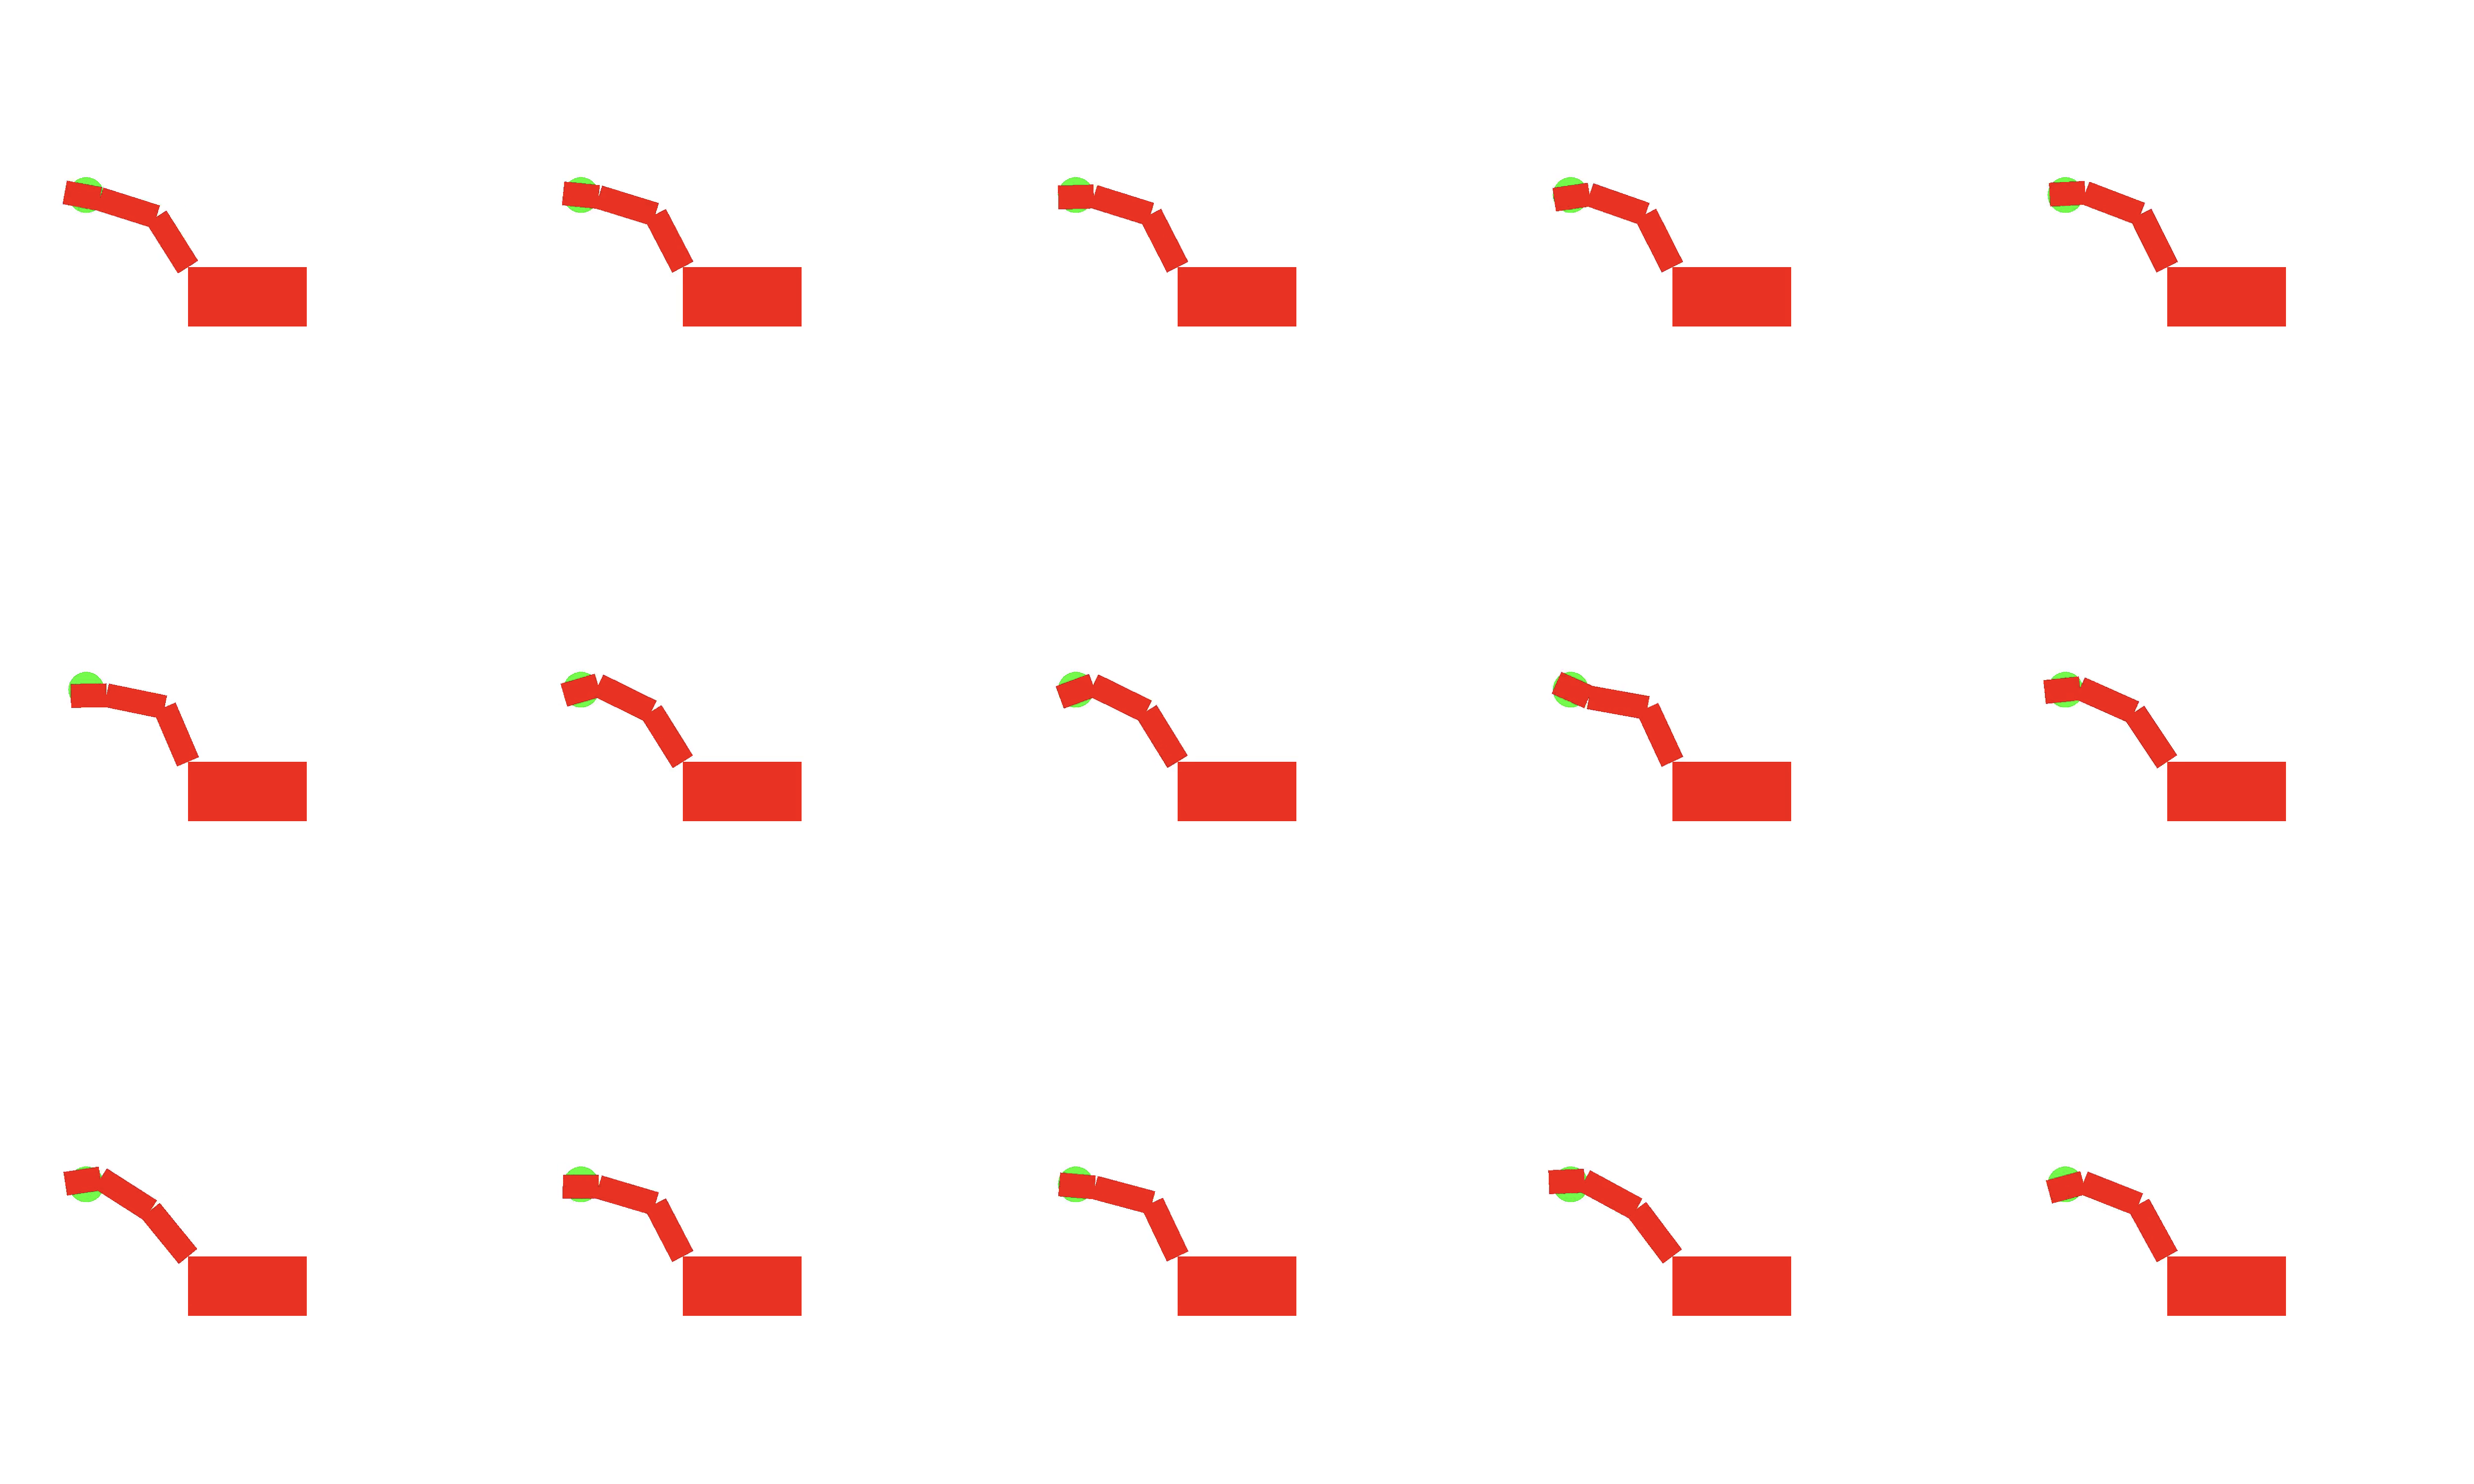
\includegraphics[width=1\textwidth]{figures/frames/frames_001.png}
      \caption{Control of a pigeon model with a static body trained on $r_{head\_stable\_manual\_reposition\_strict\_angle}$ with $max\_offset = 0.5$. The green circle indicate the margin of error around the target head location defined by $max\_offset$.}
      \label{fig:manual_trajectory_body_speed_0}
  \end{figure}

  \begin{figure}[H]
      \centering
      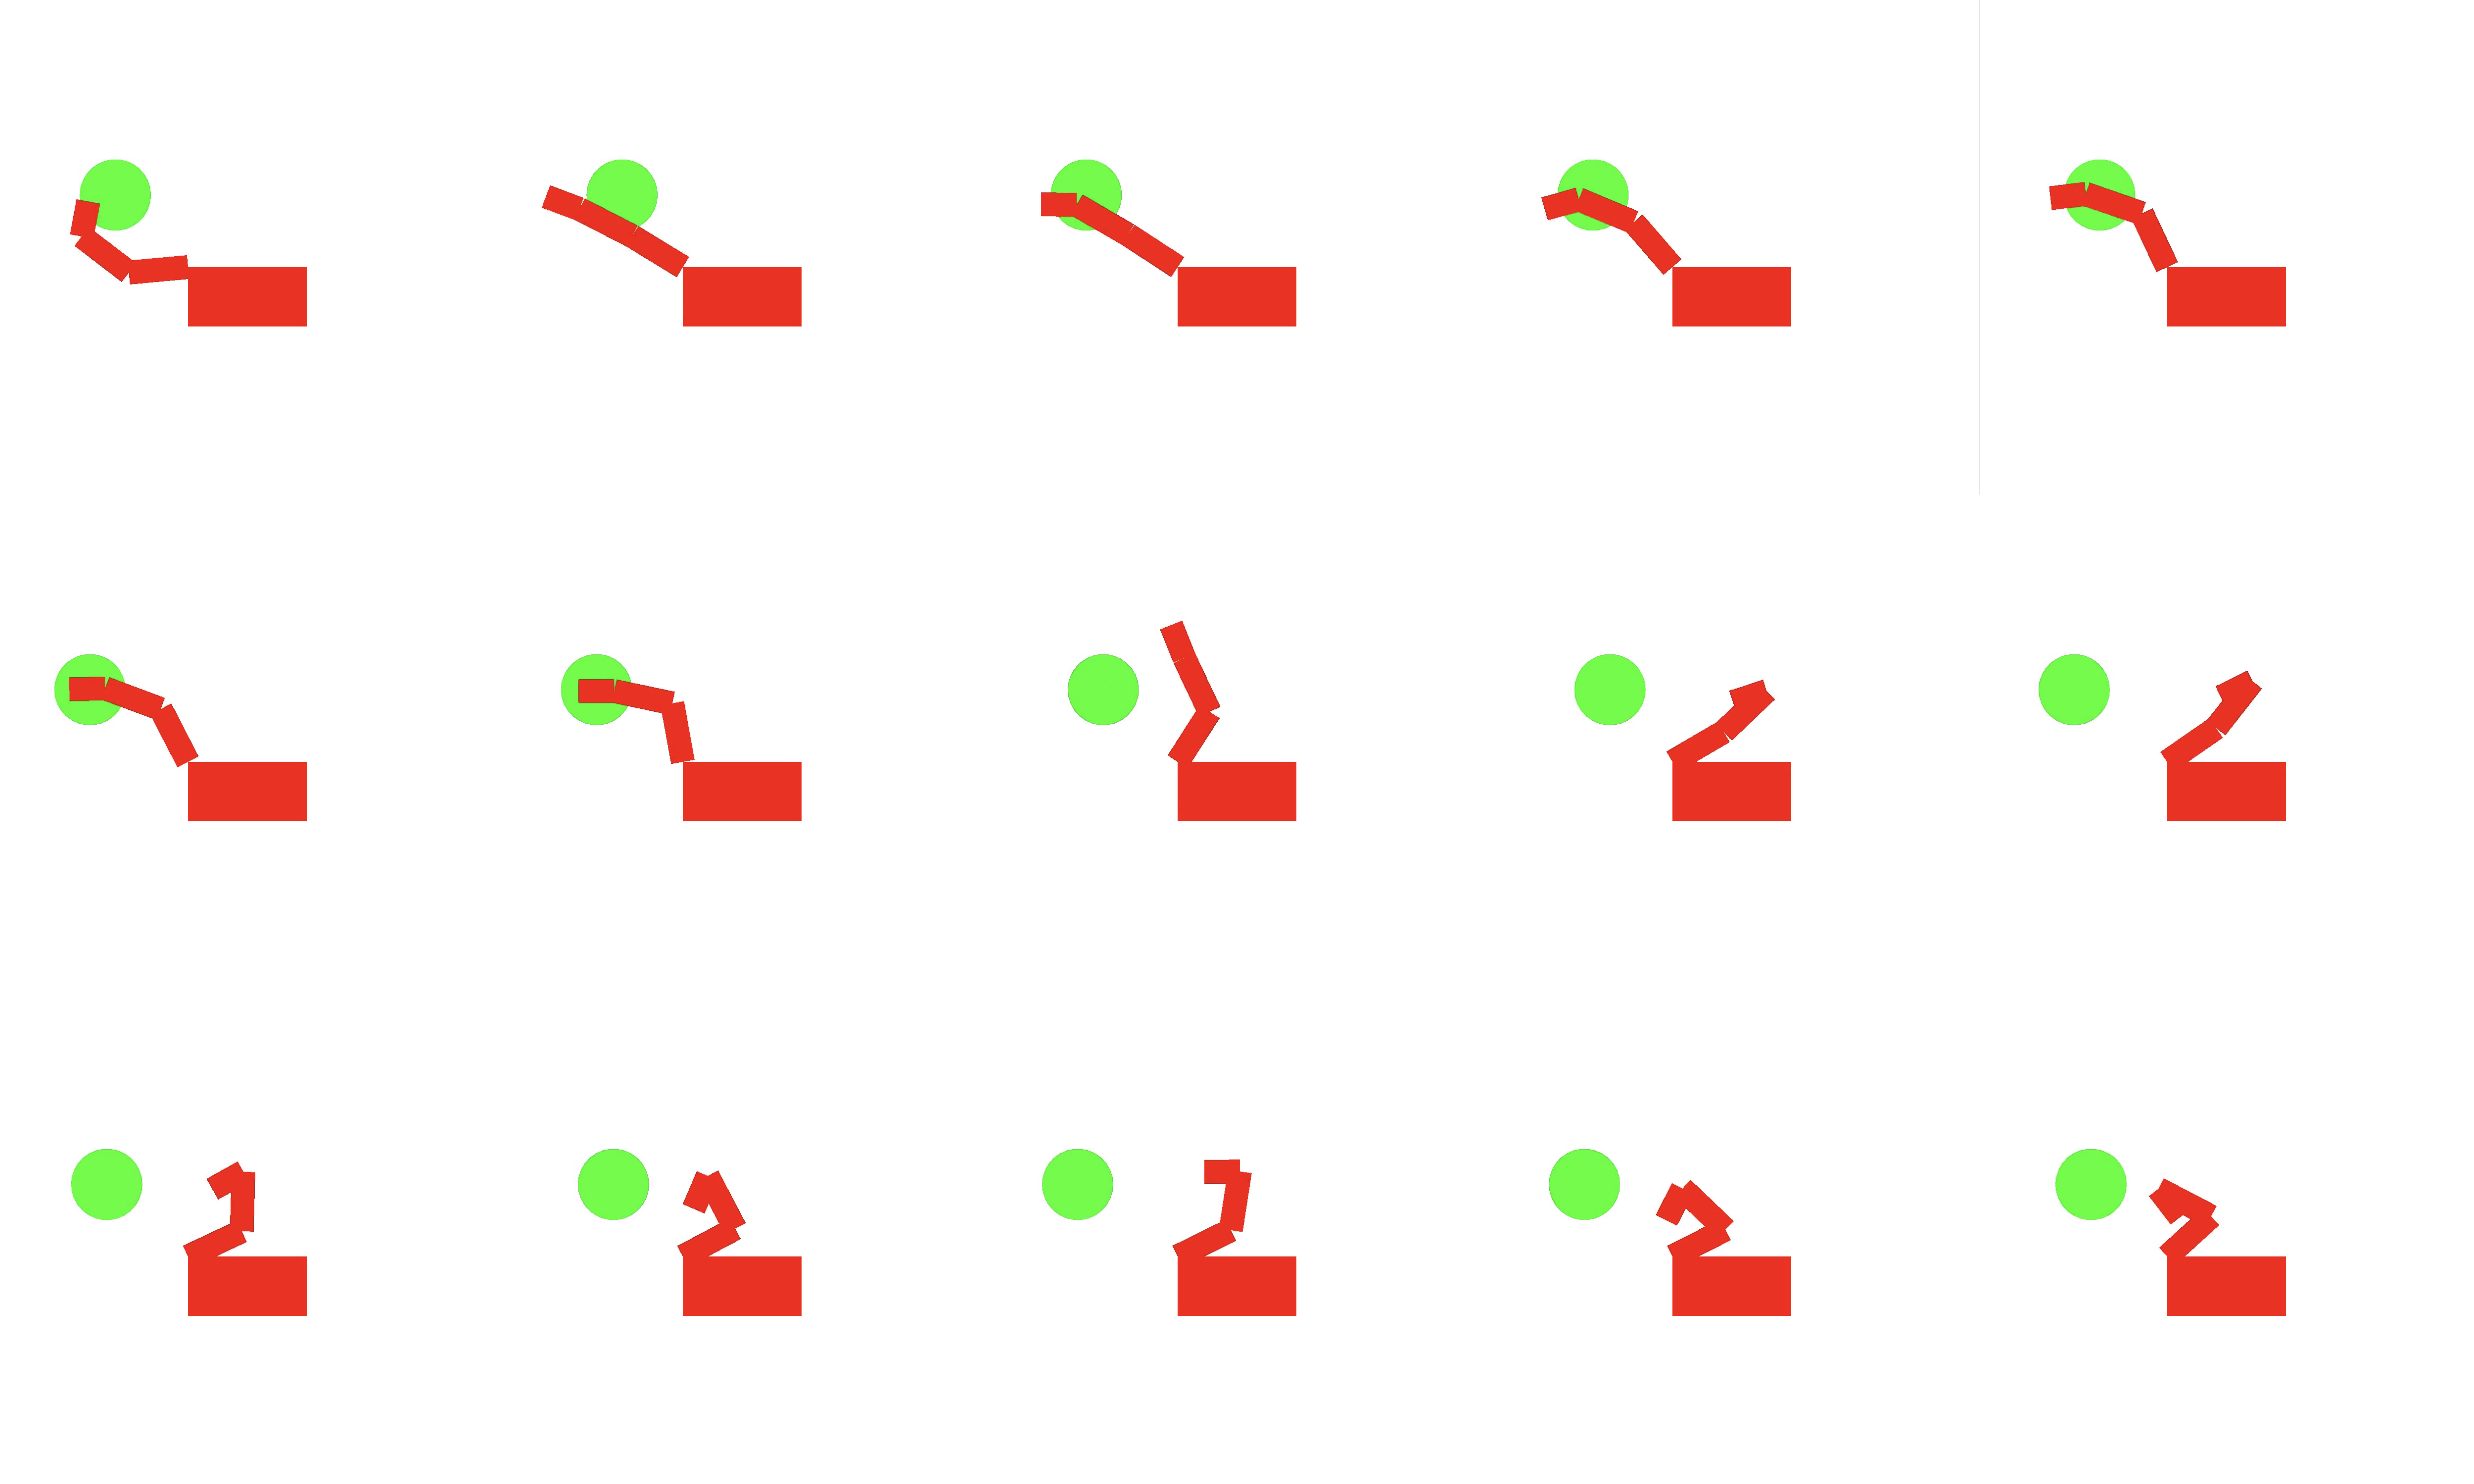
\includegraphics[width=1\textwidth]{figures/frames/frames_002.png}
      \caption{Control of a pigeon model with the body speed of 1 trained on $r_{head\_stable\_manual\_reposition\_strict\_angle}$ with $max\_offset = 1.0$. The green circle indicate the margin of error around the target head location defined by $max\_offset$.}
      \label{fig:manual_trajectory_strict_body_speed_1}
  \end{figure}

  \begin{figure}[H]
      \centering
      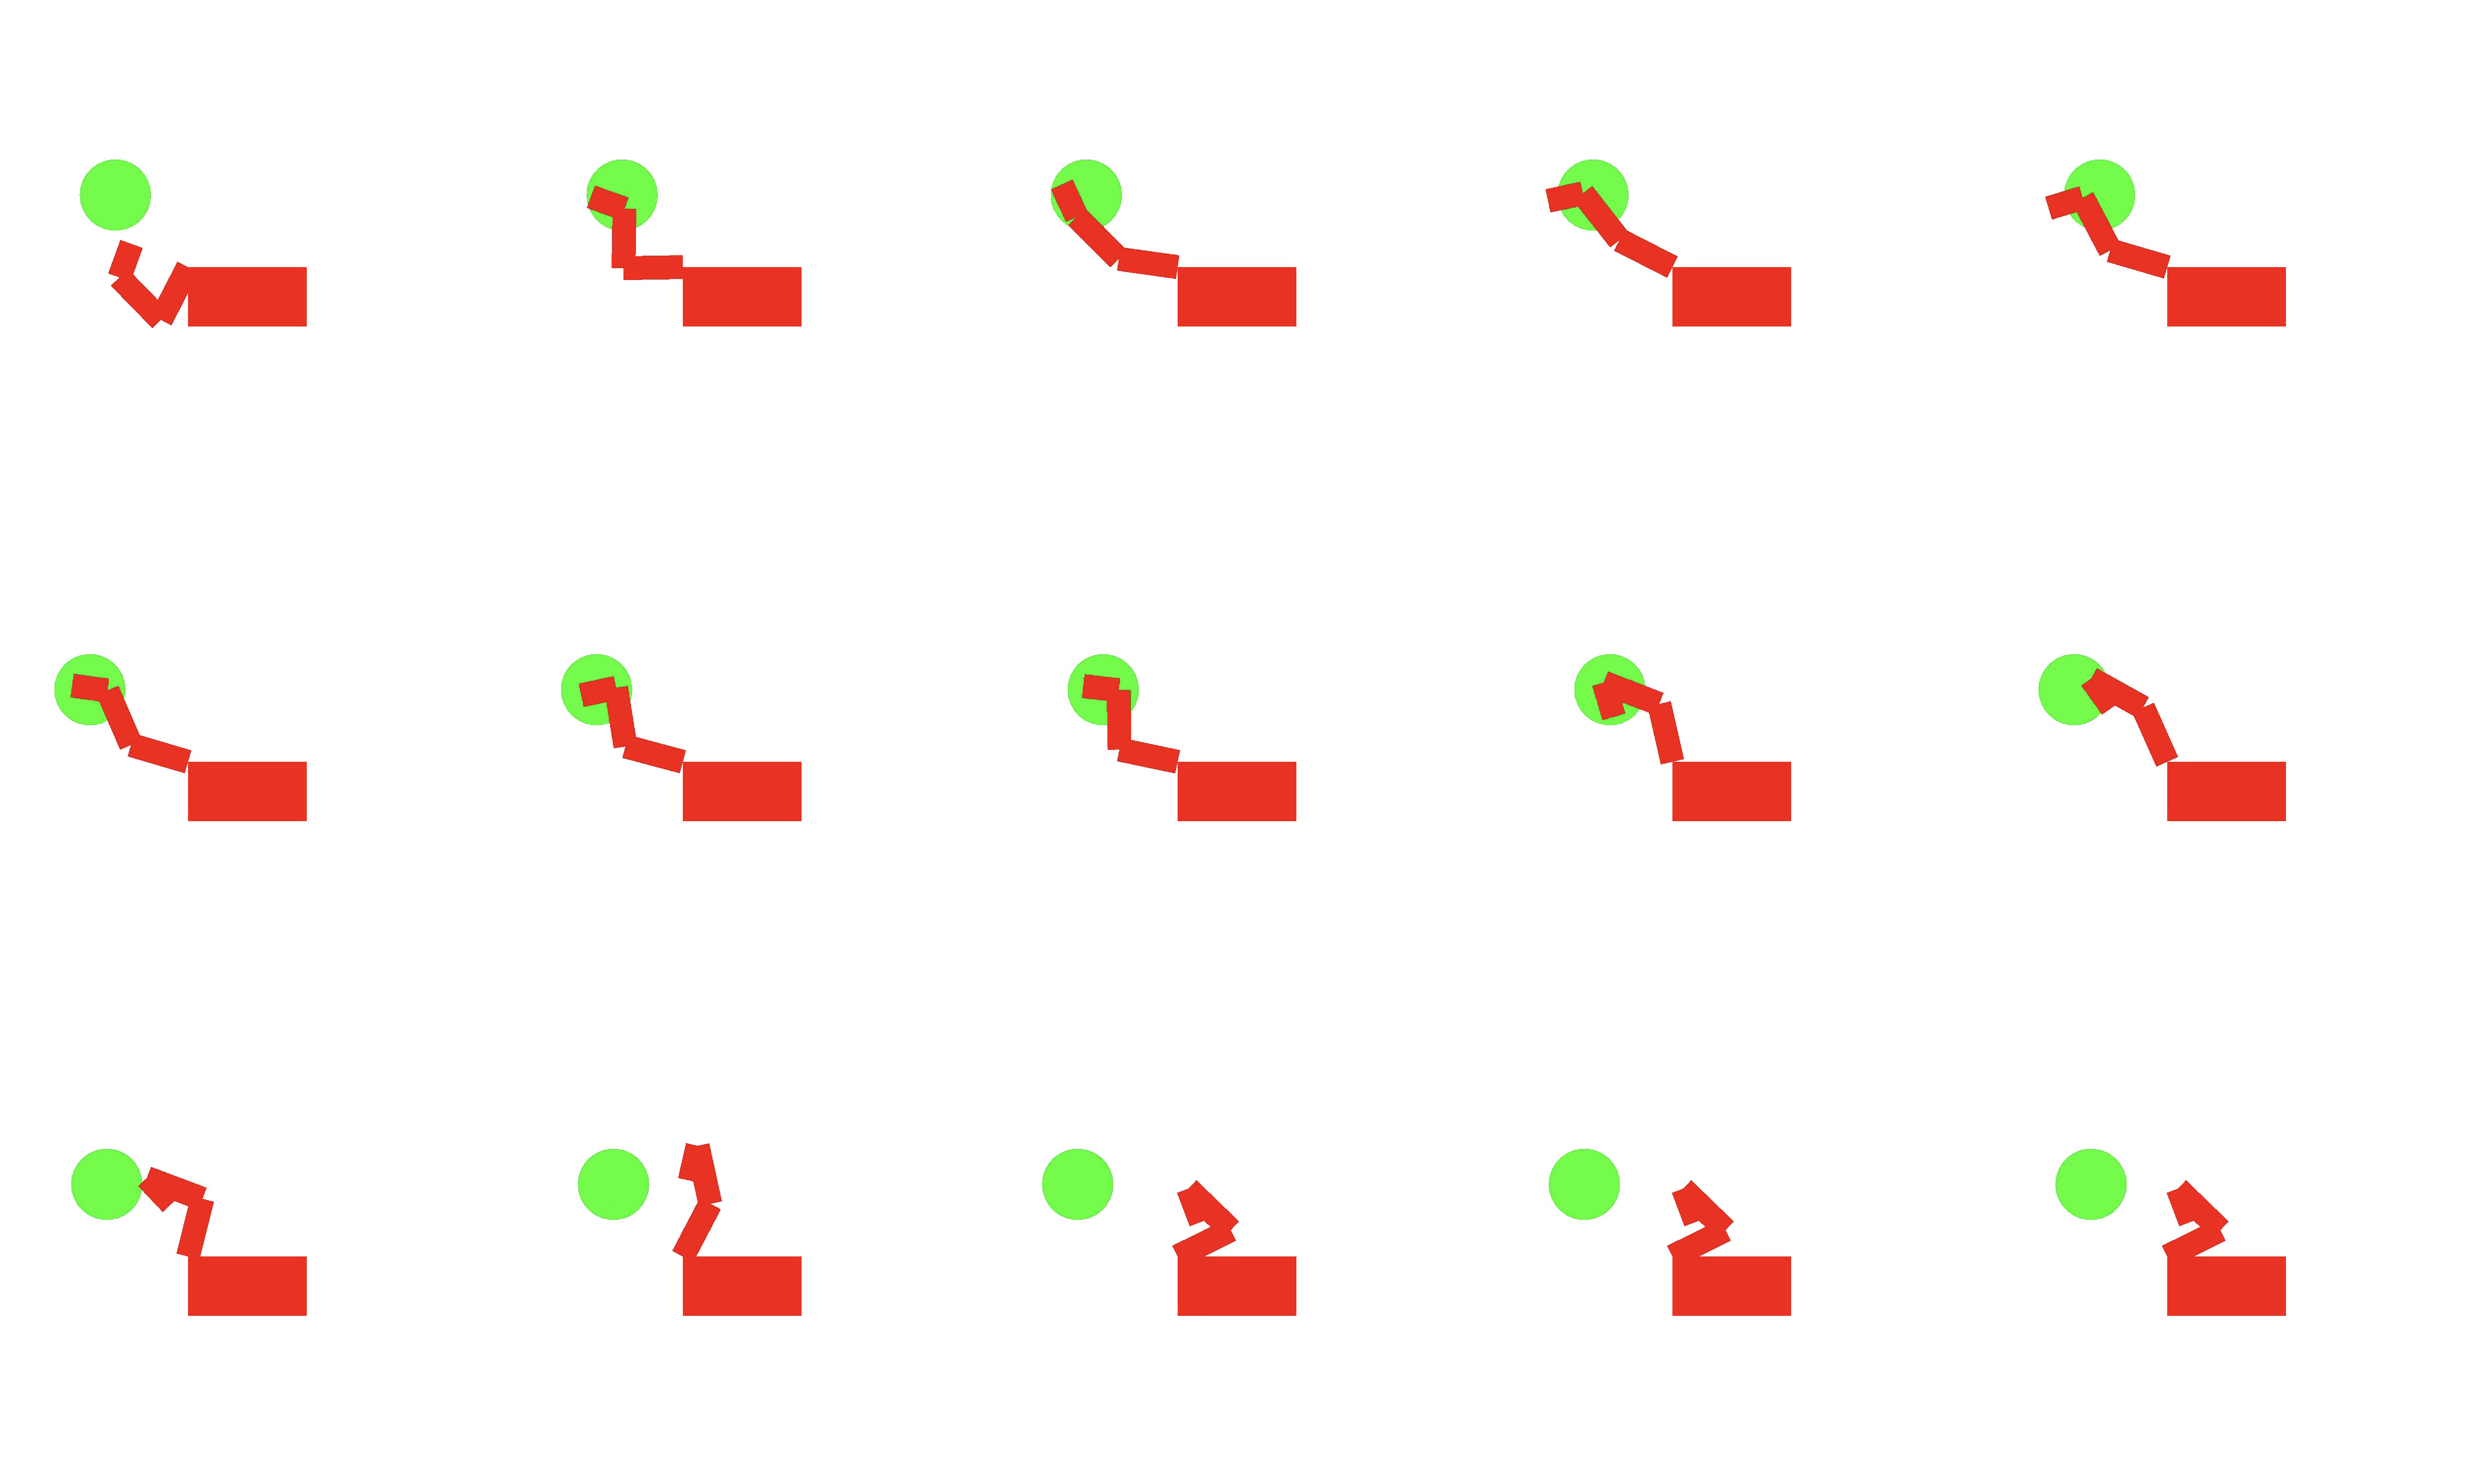
\includegraphics[width=1\textwidth]{figures/frames/frames_003.png}
      \caption{Control of a pigeon model with the body speed of 1 trained on $r_{head\_stable\_manual\_reposition}$ with $max\_offset = 1.0$. The green circle indicate the margin of error around the target head location defined by $max\_offset$.}
      \label{fig:manual_trajectory_not_strict_body_speed_1}
  \end{figure}

  \begin{figure}[H]
      \centering
      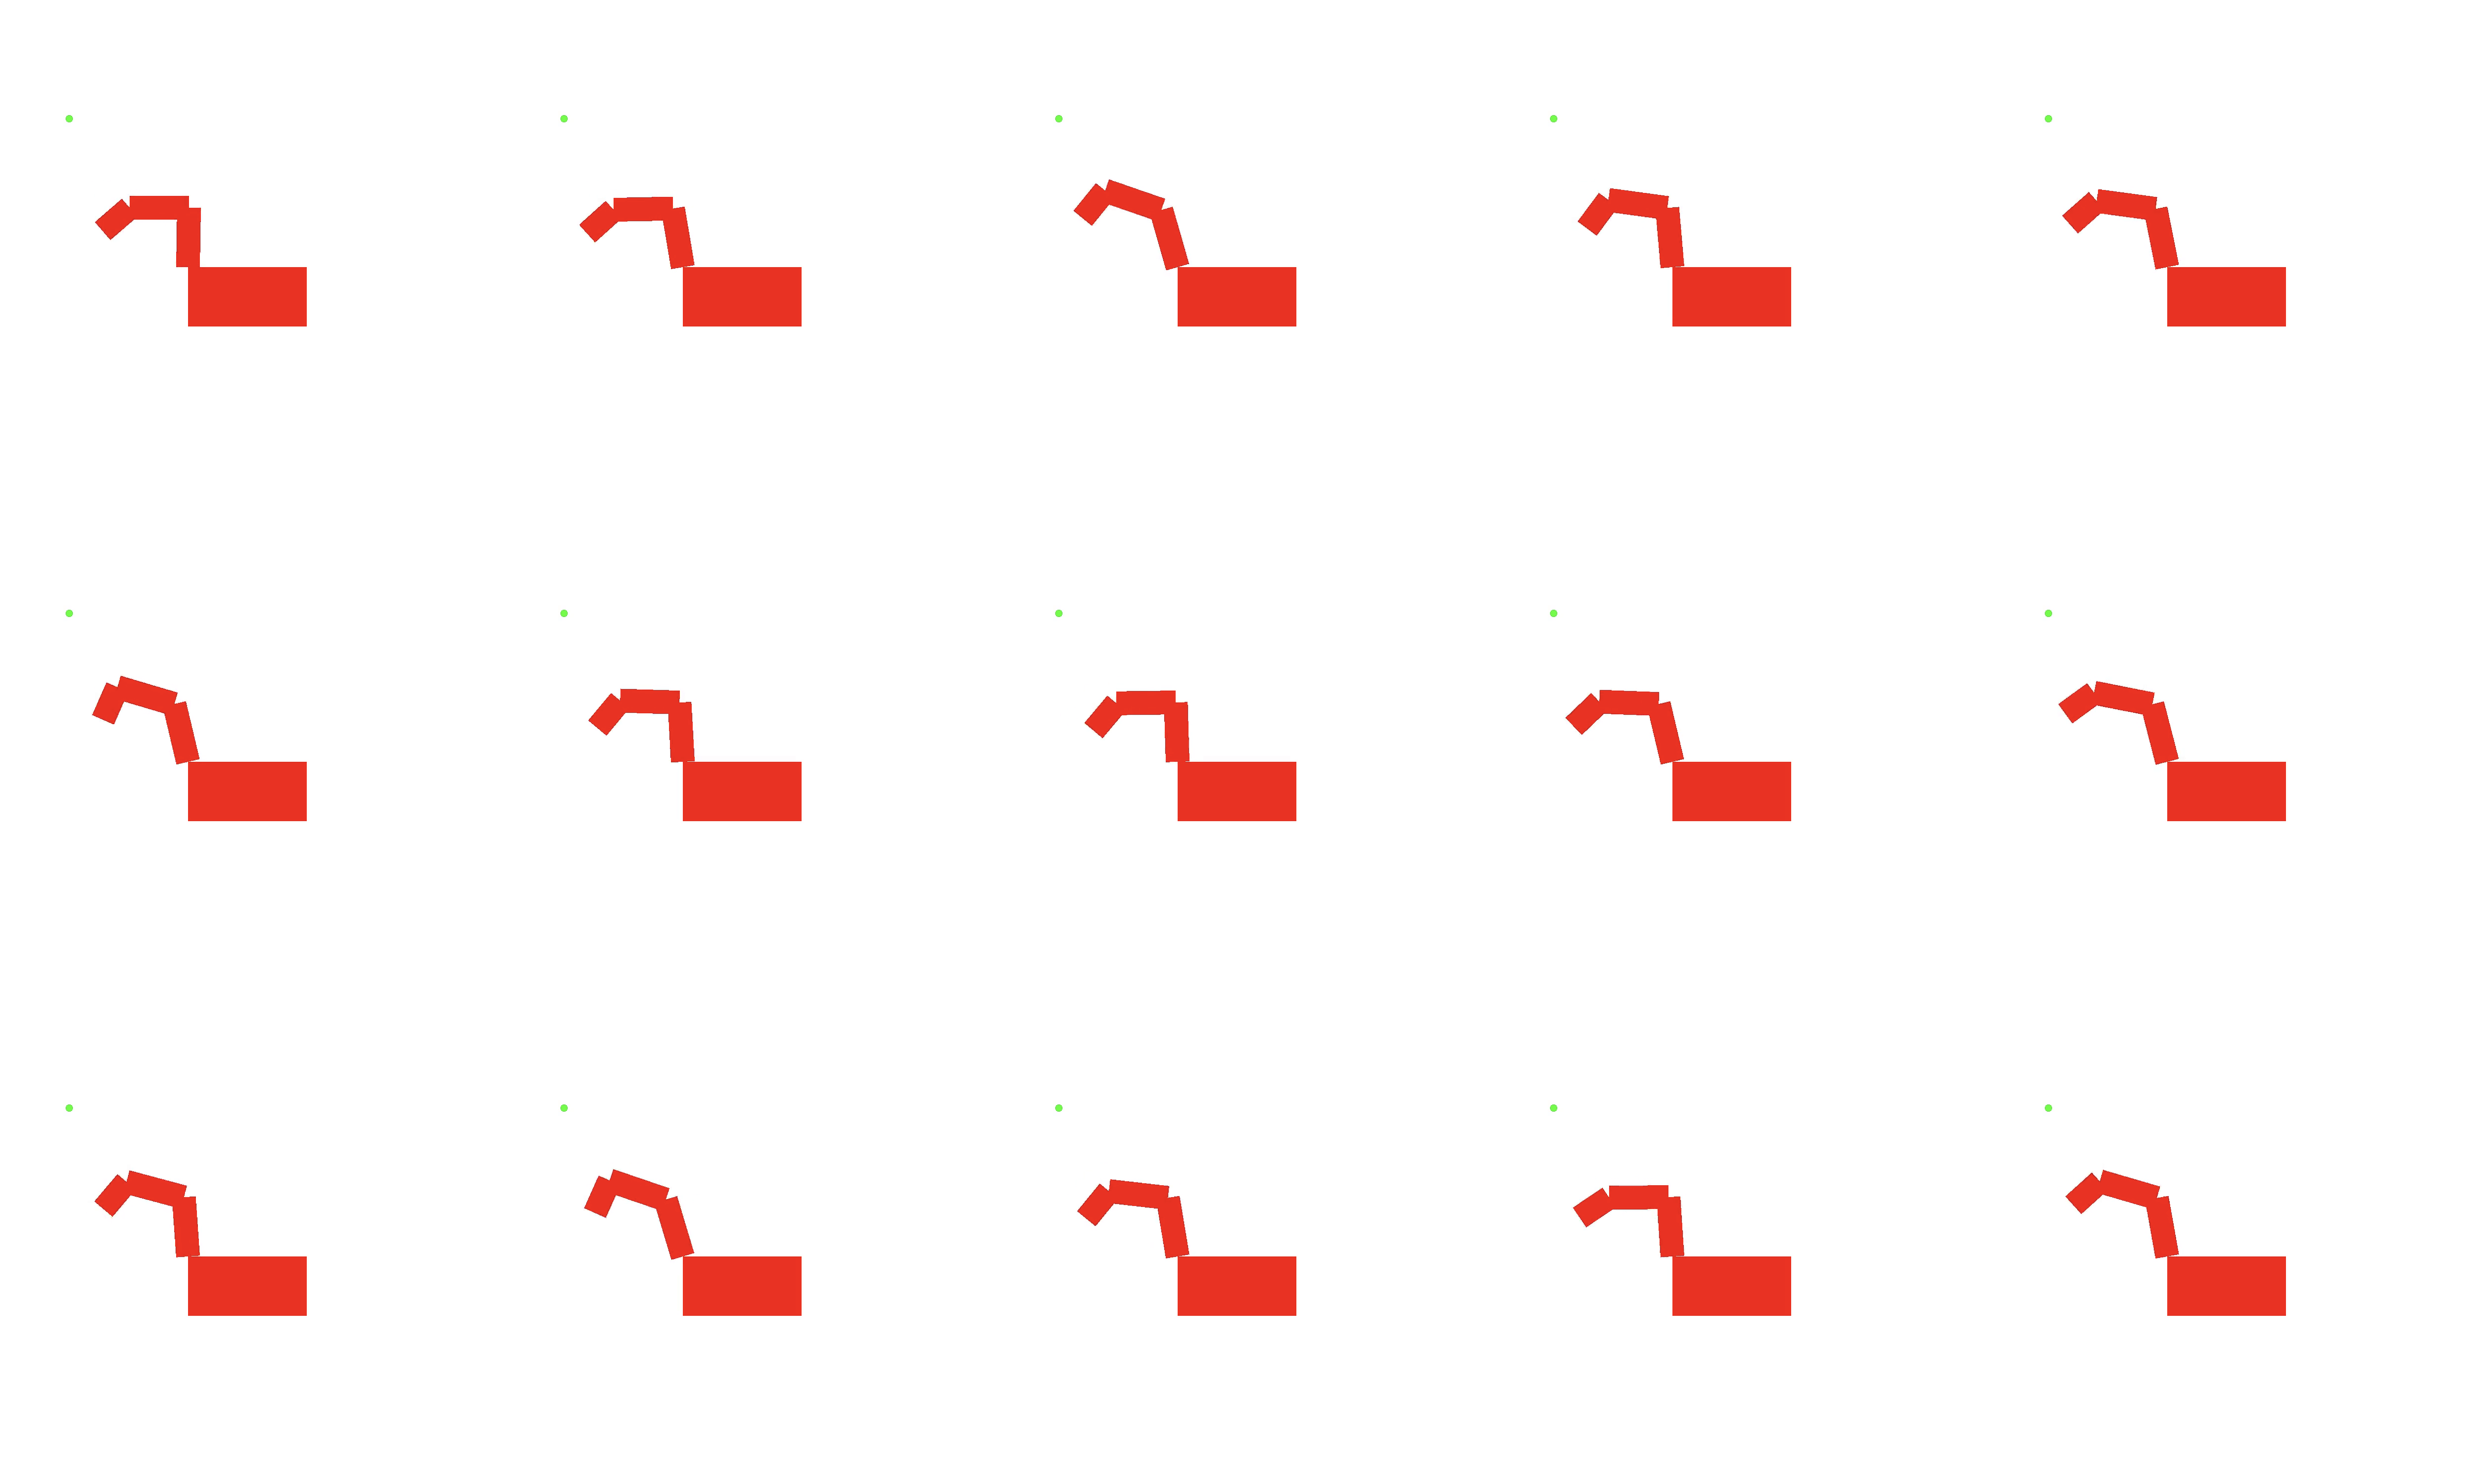
\includegraphics[width=1\textwidth]{figures/frames/frames_004.png}
      \caption{Control of a pigeon model with a static body trained on $r_{fifty\_fifty}$}
      \label{fig:fifty_fifty_body_speed_0}
  \end{figure}

  \begin{figure}[H]
      \centering
      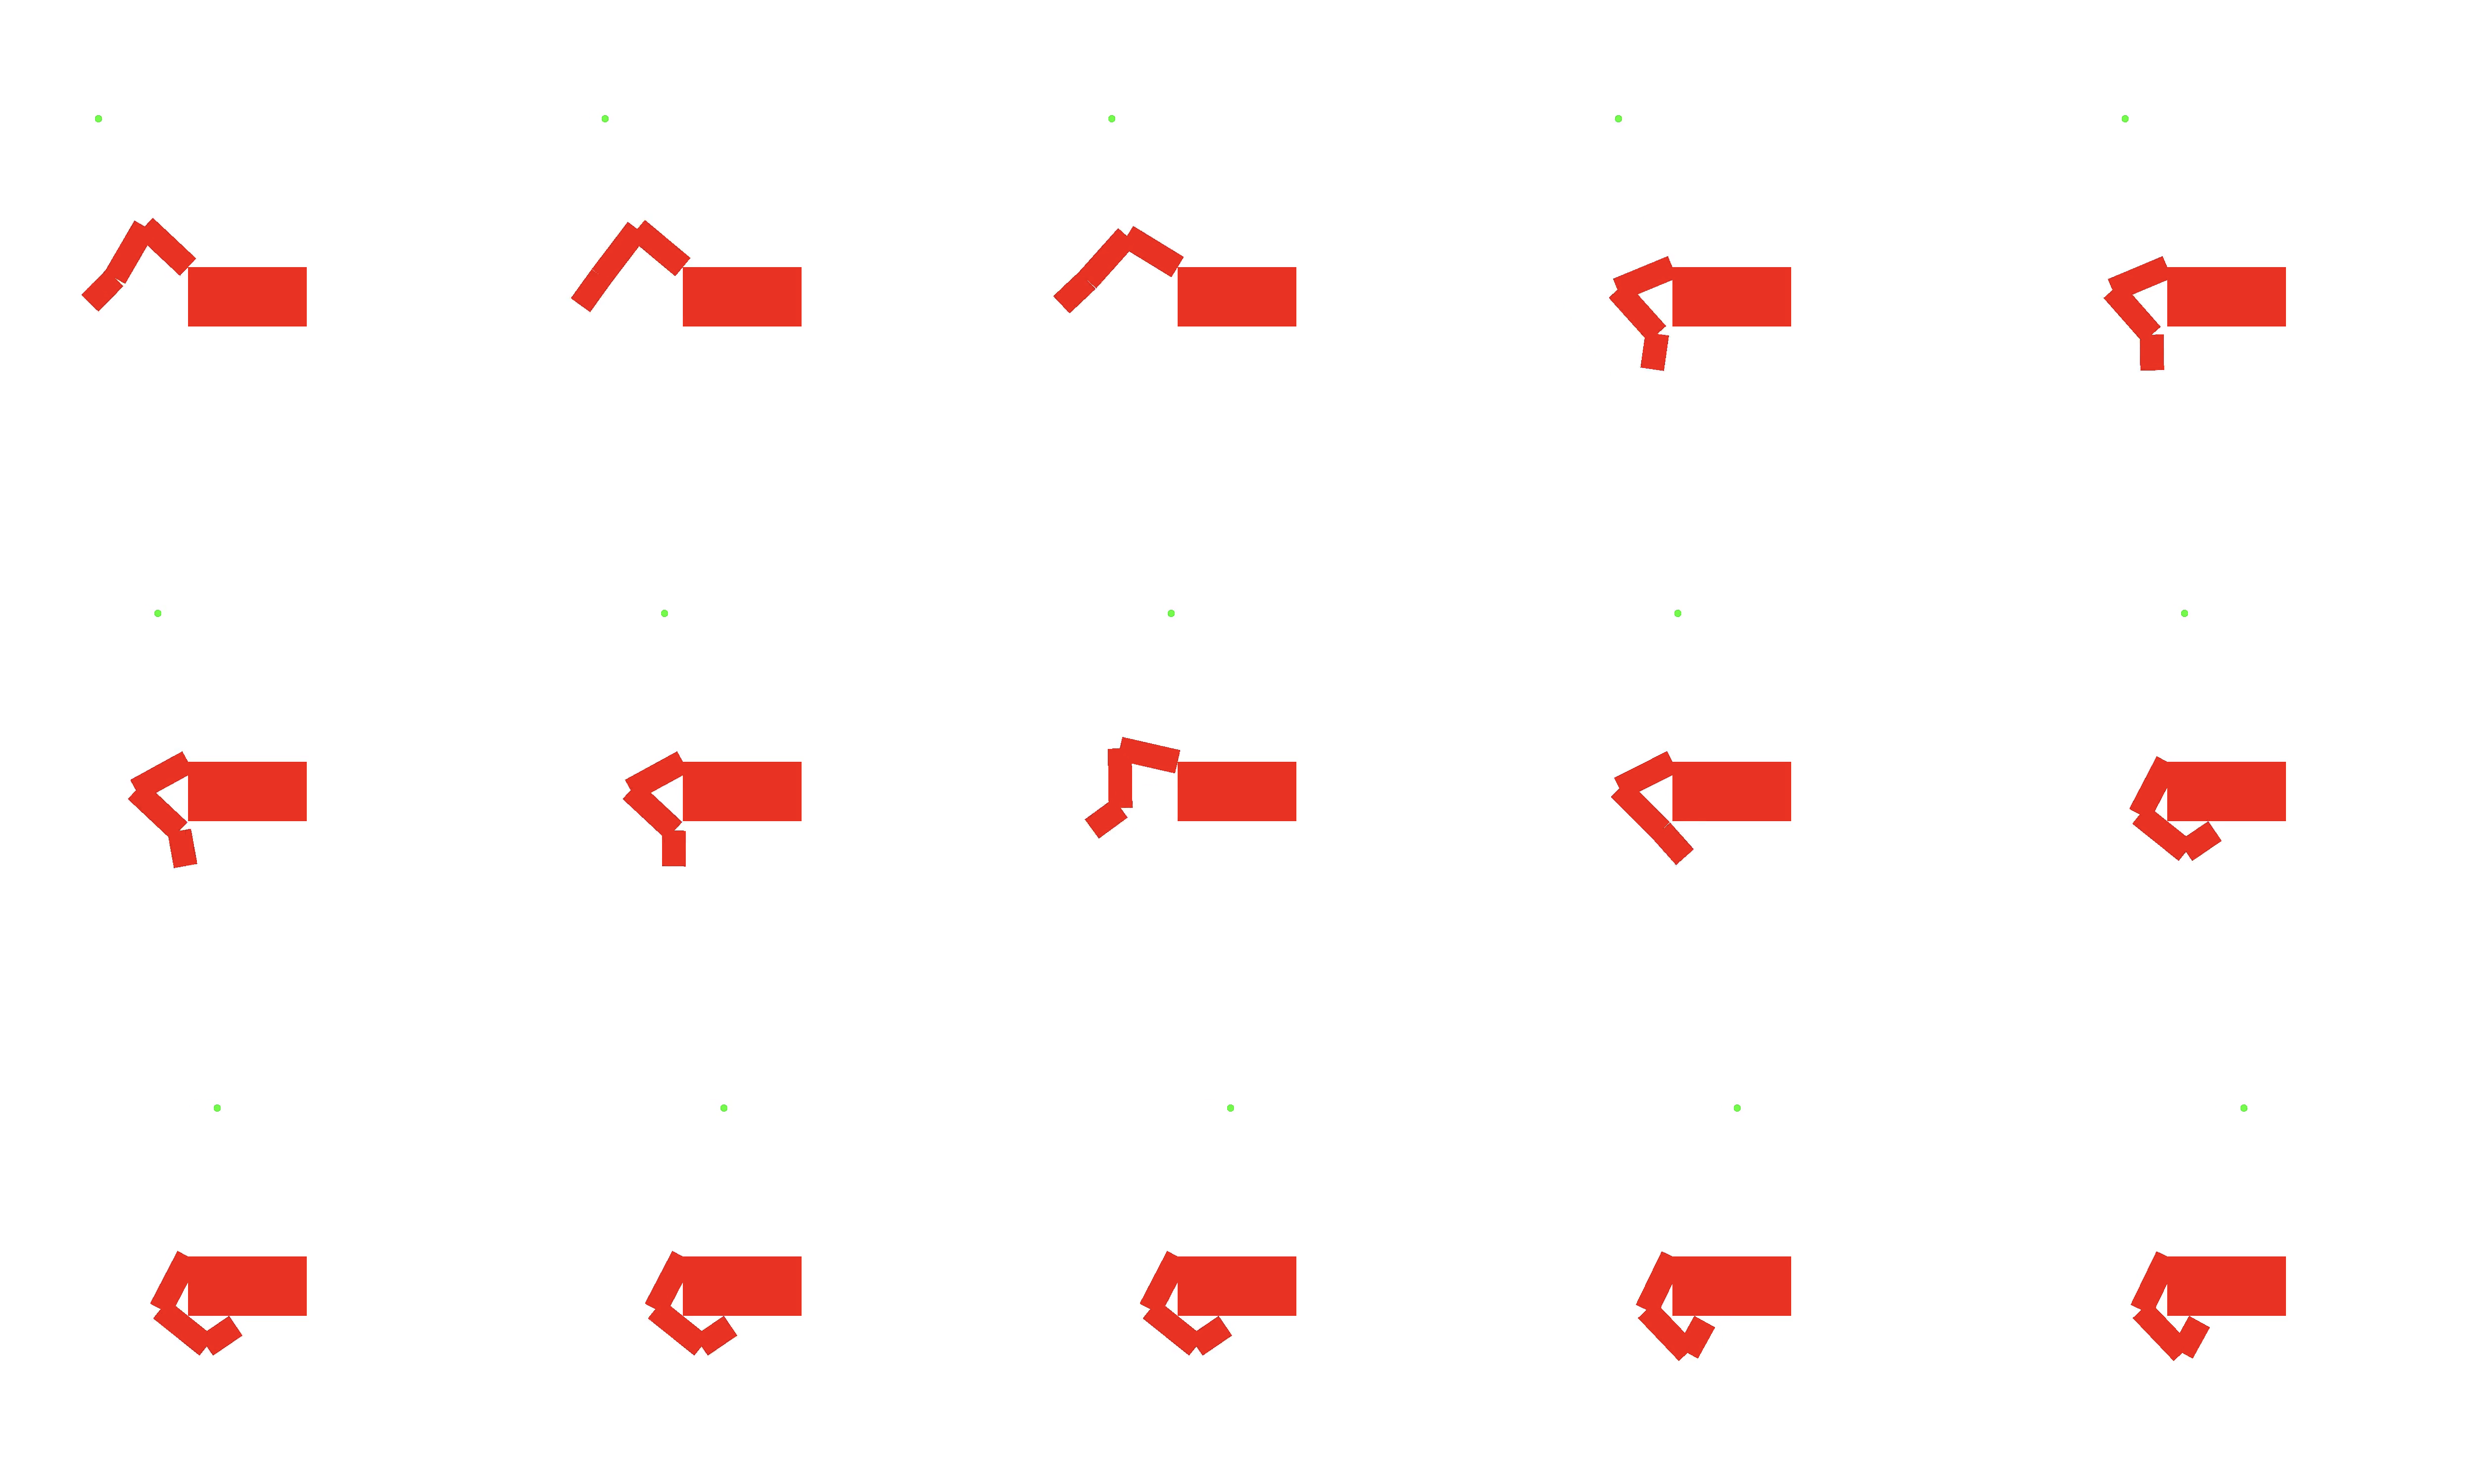
\includegraphics[width=1\textwidth]{figures/frames/frames_005.png}
      \caption{Control of a pigeon model with the body speed of 1 trained on $r_{fifty\_fifty}$}
      \label{fig:fifty_fifty_body_speed_1}
  \end{figure}

% figures of pigeon head trajectories
\section{Head Trajectories}
% explanation
  We additionally visualized the trajectories of heads and bodies of each pigeon model. With this method, we can compare the resulting behaviors of the controlled pigeons between the reward functions they were trained on.

  We coupled the trajectories produced by pigeons with the same body speeds in \ref{fig:head_bs_0} and \ref{fig:head_bs_1_all}.

  \begin{figure}[H]
      \centering
      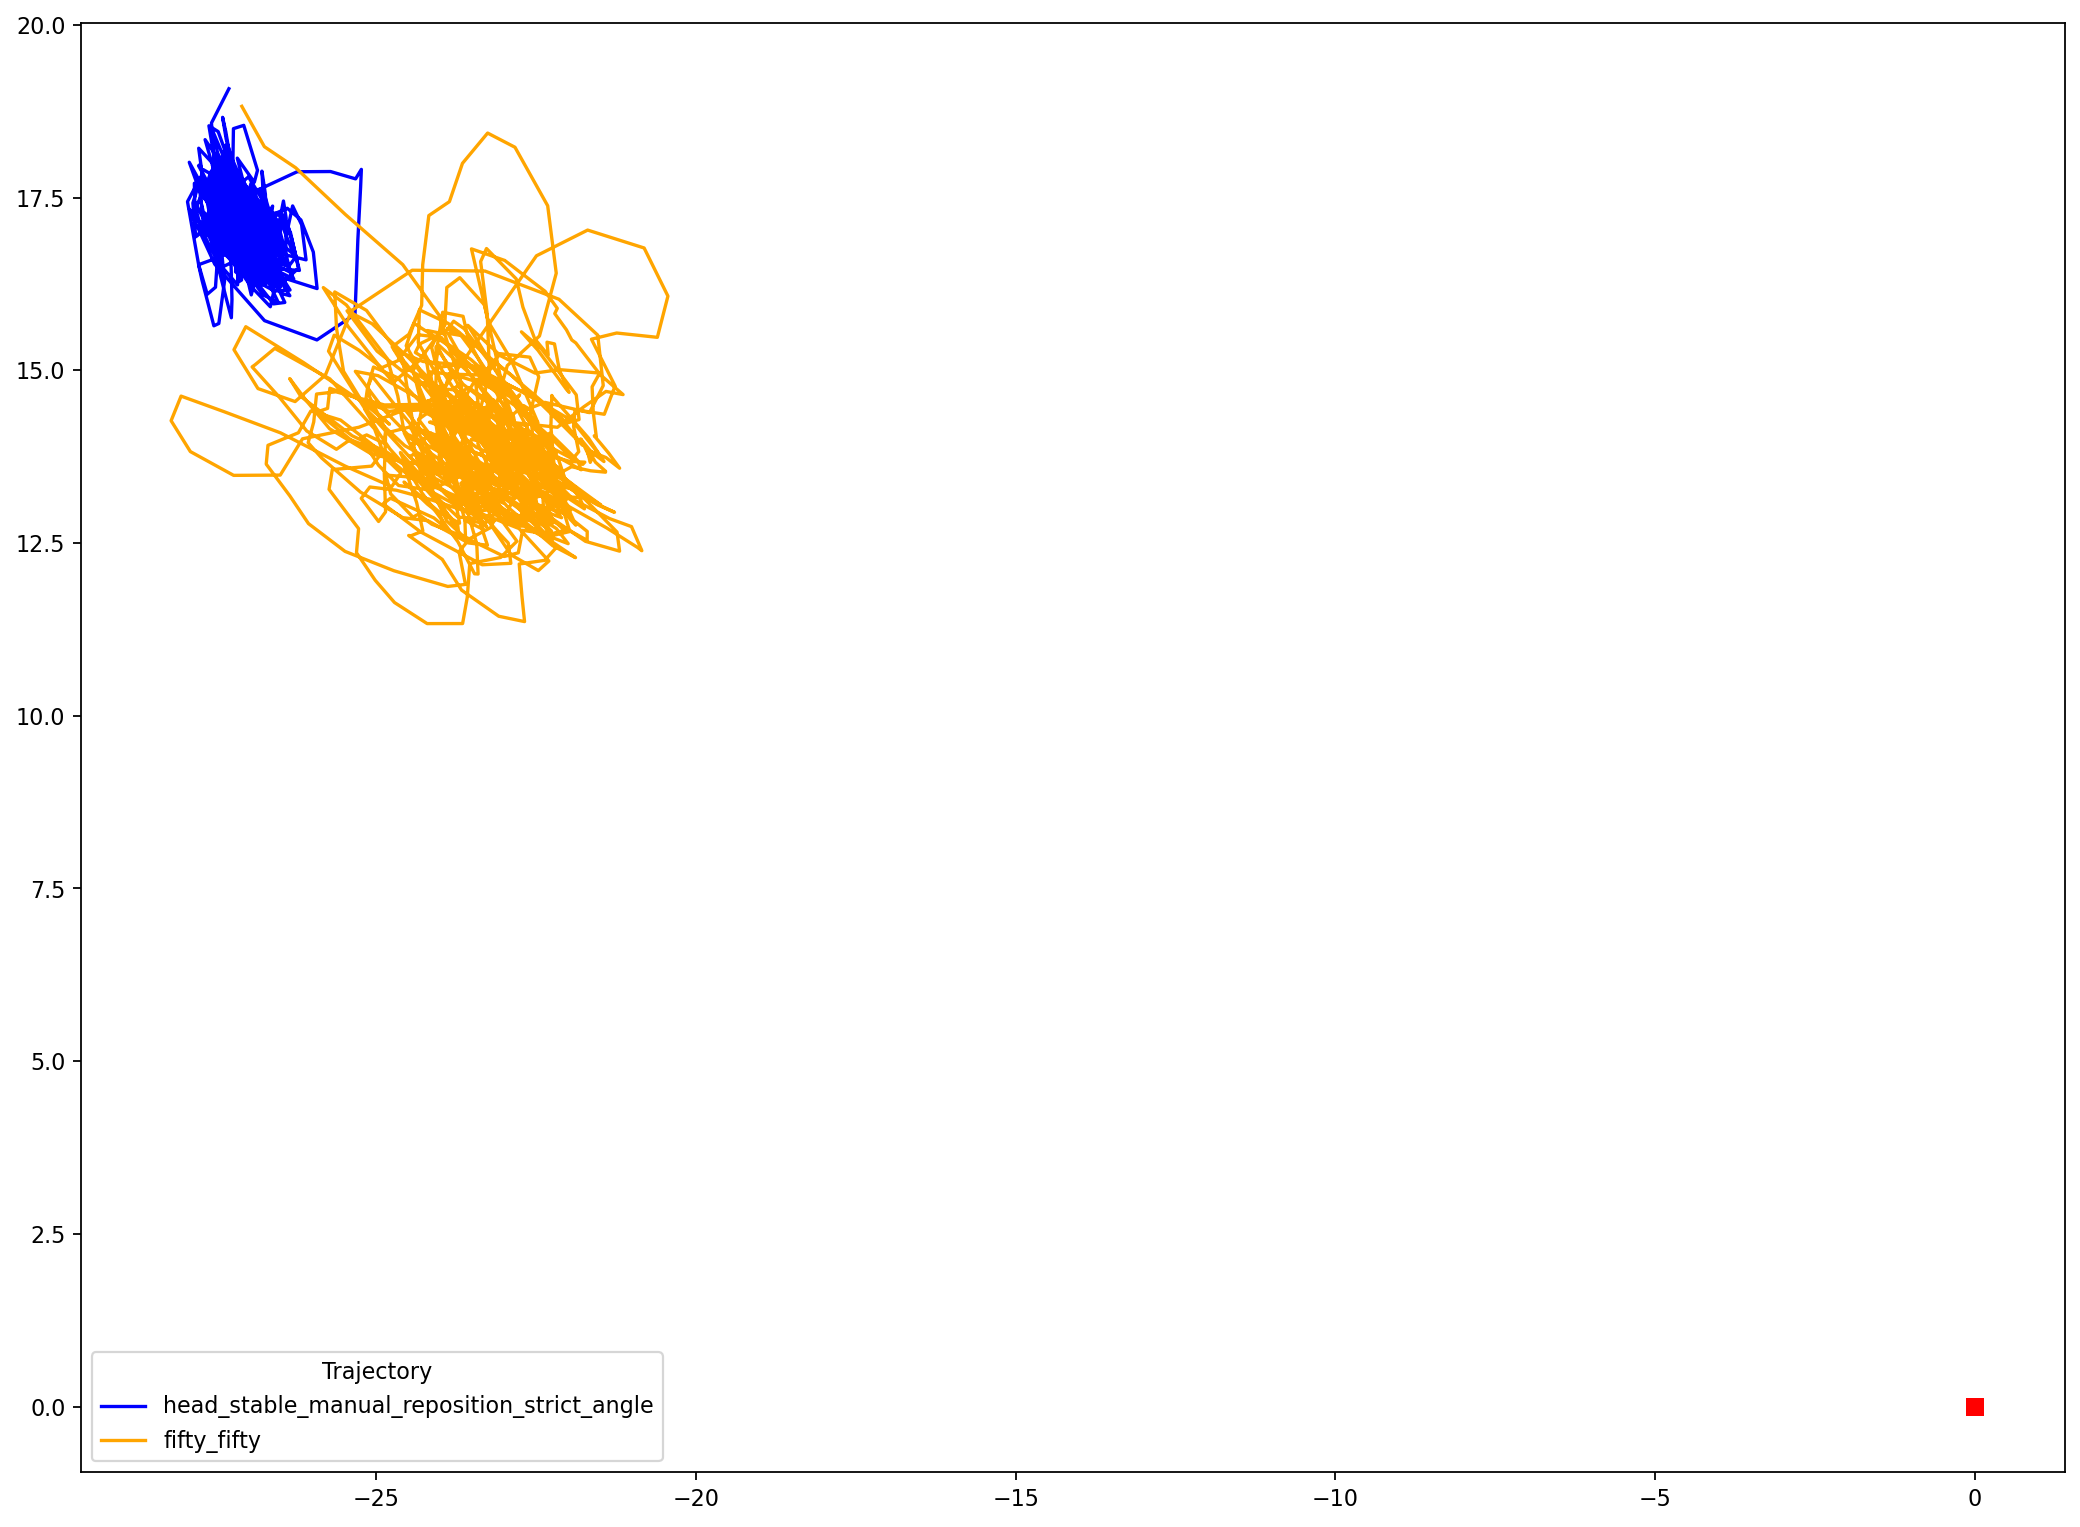
\includegraphics[width=1\textwidth]{figures/head_tracking_results/pigeon_bs_0.png}
      \caption{Trajectories of heads and bodies of pigeon models with static bodies trained on $r_{head\_stable\_manual\_reposition\_strict\_angle}$ with $max\_offset = 0.5$ and $r_{fifty\_fifty}$}
      \label{fig:head_bs_0}
  \end{figure}

  \begin{figure}[H]
      \centering
      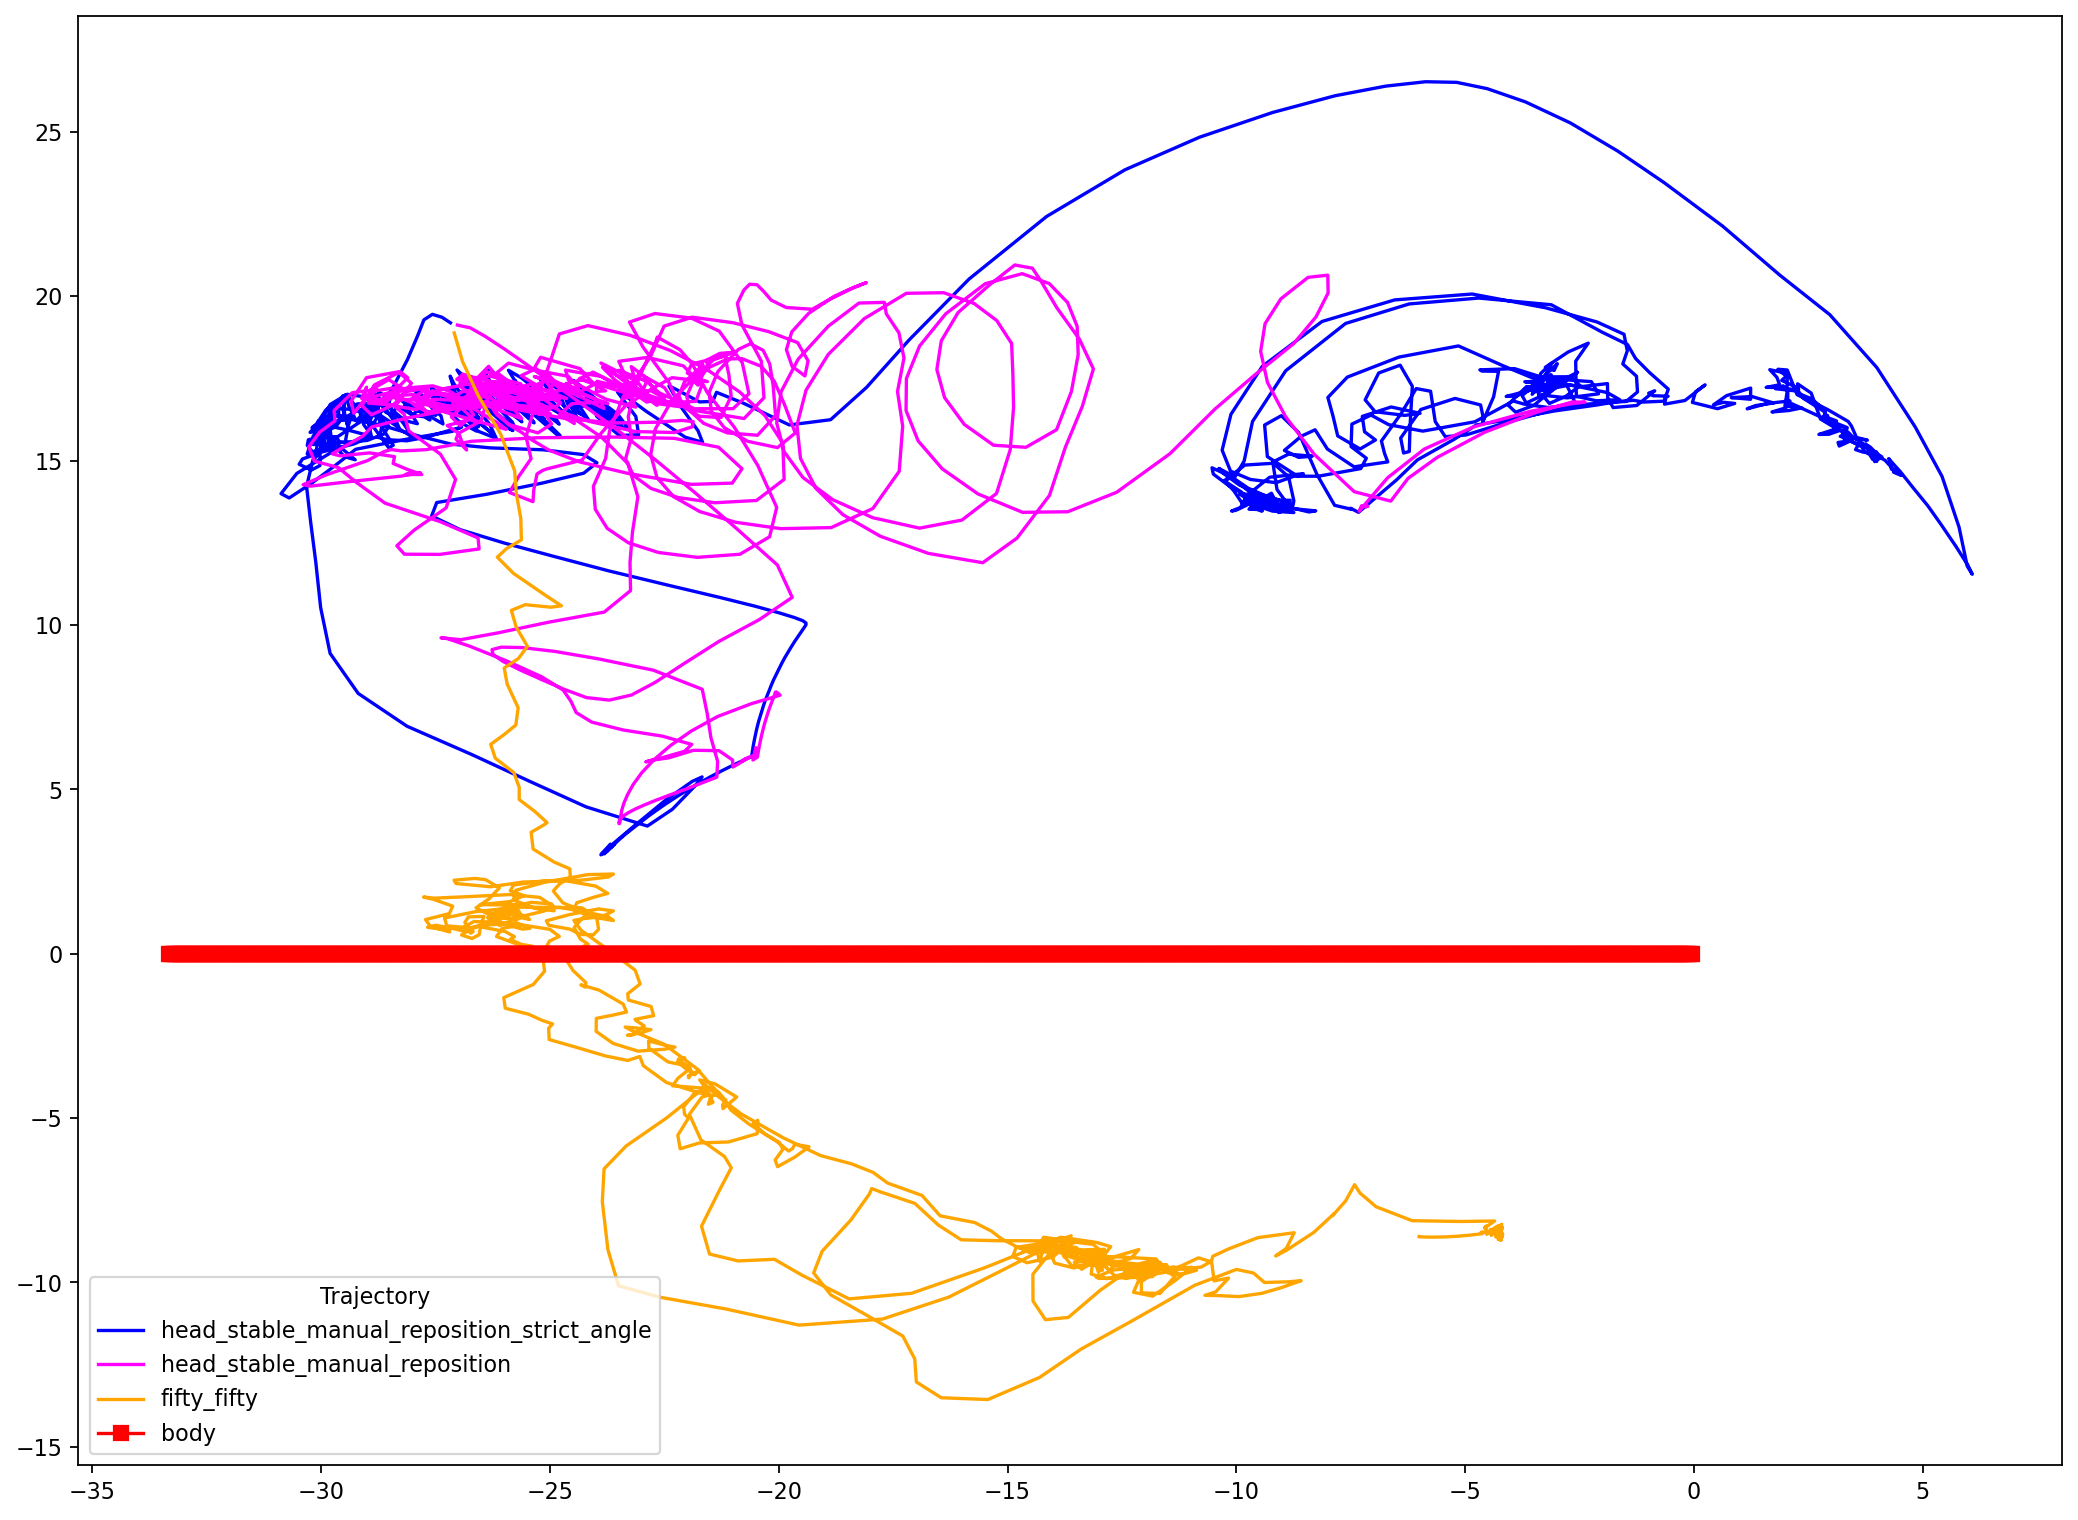
\includegraphics[width=1\textwidth]{figures/head_tracking_results/pigeon_bs_1_all.png}
      \caption{Trajectories of heads and bodies of pigeon models with body speeds of 1 trained on $r_{head\_stable\_manual\_reposition\_strict\_angle}$ with $max\_offset = 1.0$, $r_{head\_stable\_manual\_reposition}$ with $max\_offset = 1.0$, and $r_{fifty\_fifty}$}
      \label{fig:head_bs_1_all}
  \end{figure}

  For pigeon models with static bodies, the manually-defined trajectory set by $r_{head\_stable\_manual\_reposition\_strict\_angle}$ and the trajectory that reflects the preliminary hypotheses set by $r_{fifty\_fifty}$ are similar: they both attempt to stabilize the head in one location. The trajectory produced by the controller trained on $r_{fifty\_fifty}$, albeit with more variance, has such trait as an emergent behavior.

  For pigeon models with body speeds of 1, as mentioned beforehand, pigeon models whose controllers were trained using $r_{head\_stable\_manual\_reposition\_strict\_angle}$ and $r_{head\_stable\_manual\_reposition}$ struggle to maintain their heads to follow their target locations $T$.
  The manually-defined trajectories set by the two reward functions reflect such behaviors.

  Taking these issues into consideration, we present an alternative visualization of the trajectories \ref{fig:head_bs_1_all_trimmed}, where the trajectory representing $r_{head\_stable\_manual\_reposition\_strict\_angle}$ is trimmed to only show from 250 to 500 timesteps and the trajectory representing $r_{head\_stable\_manual\_reposition}$ is trimmed to only show from 300 to 500 timesteps.
  The two manually-defined trajectories now share similar paths of head-bobbing; however even with such adjustments, it is evident that the trajectory produced by the controller trained on $r_{fifty\_fifty}$ is vastly different from the 2 prior trajectories.

  \begin{figure}[H]
      \centering
      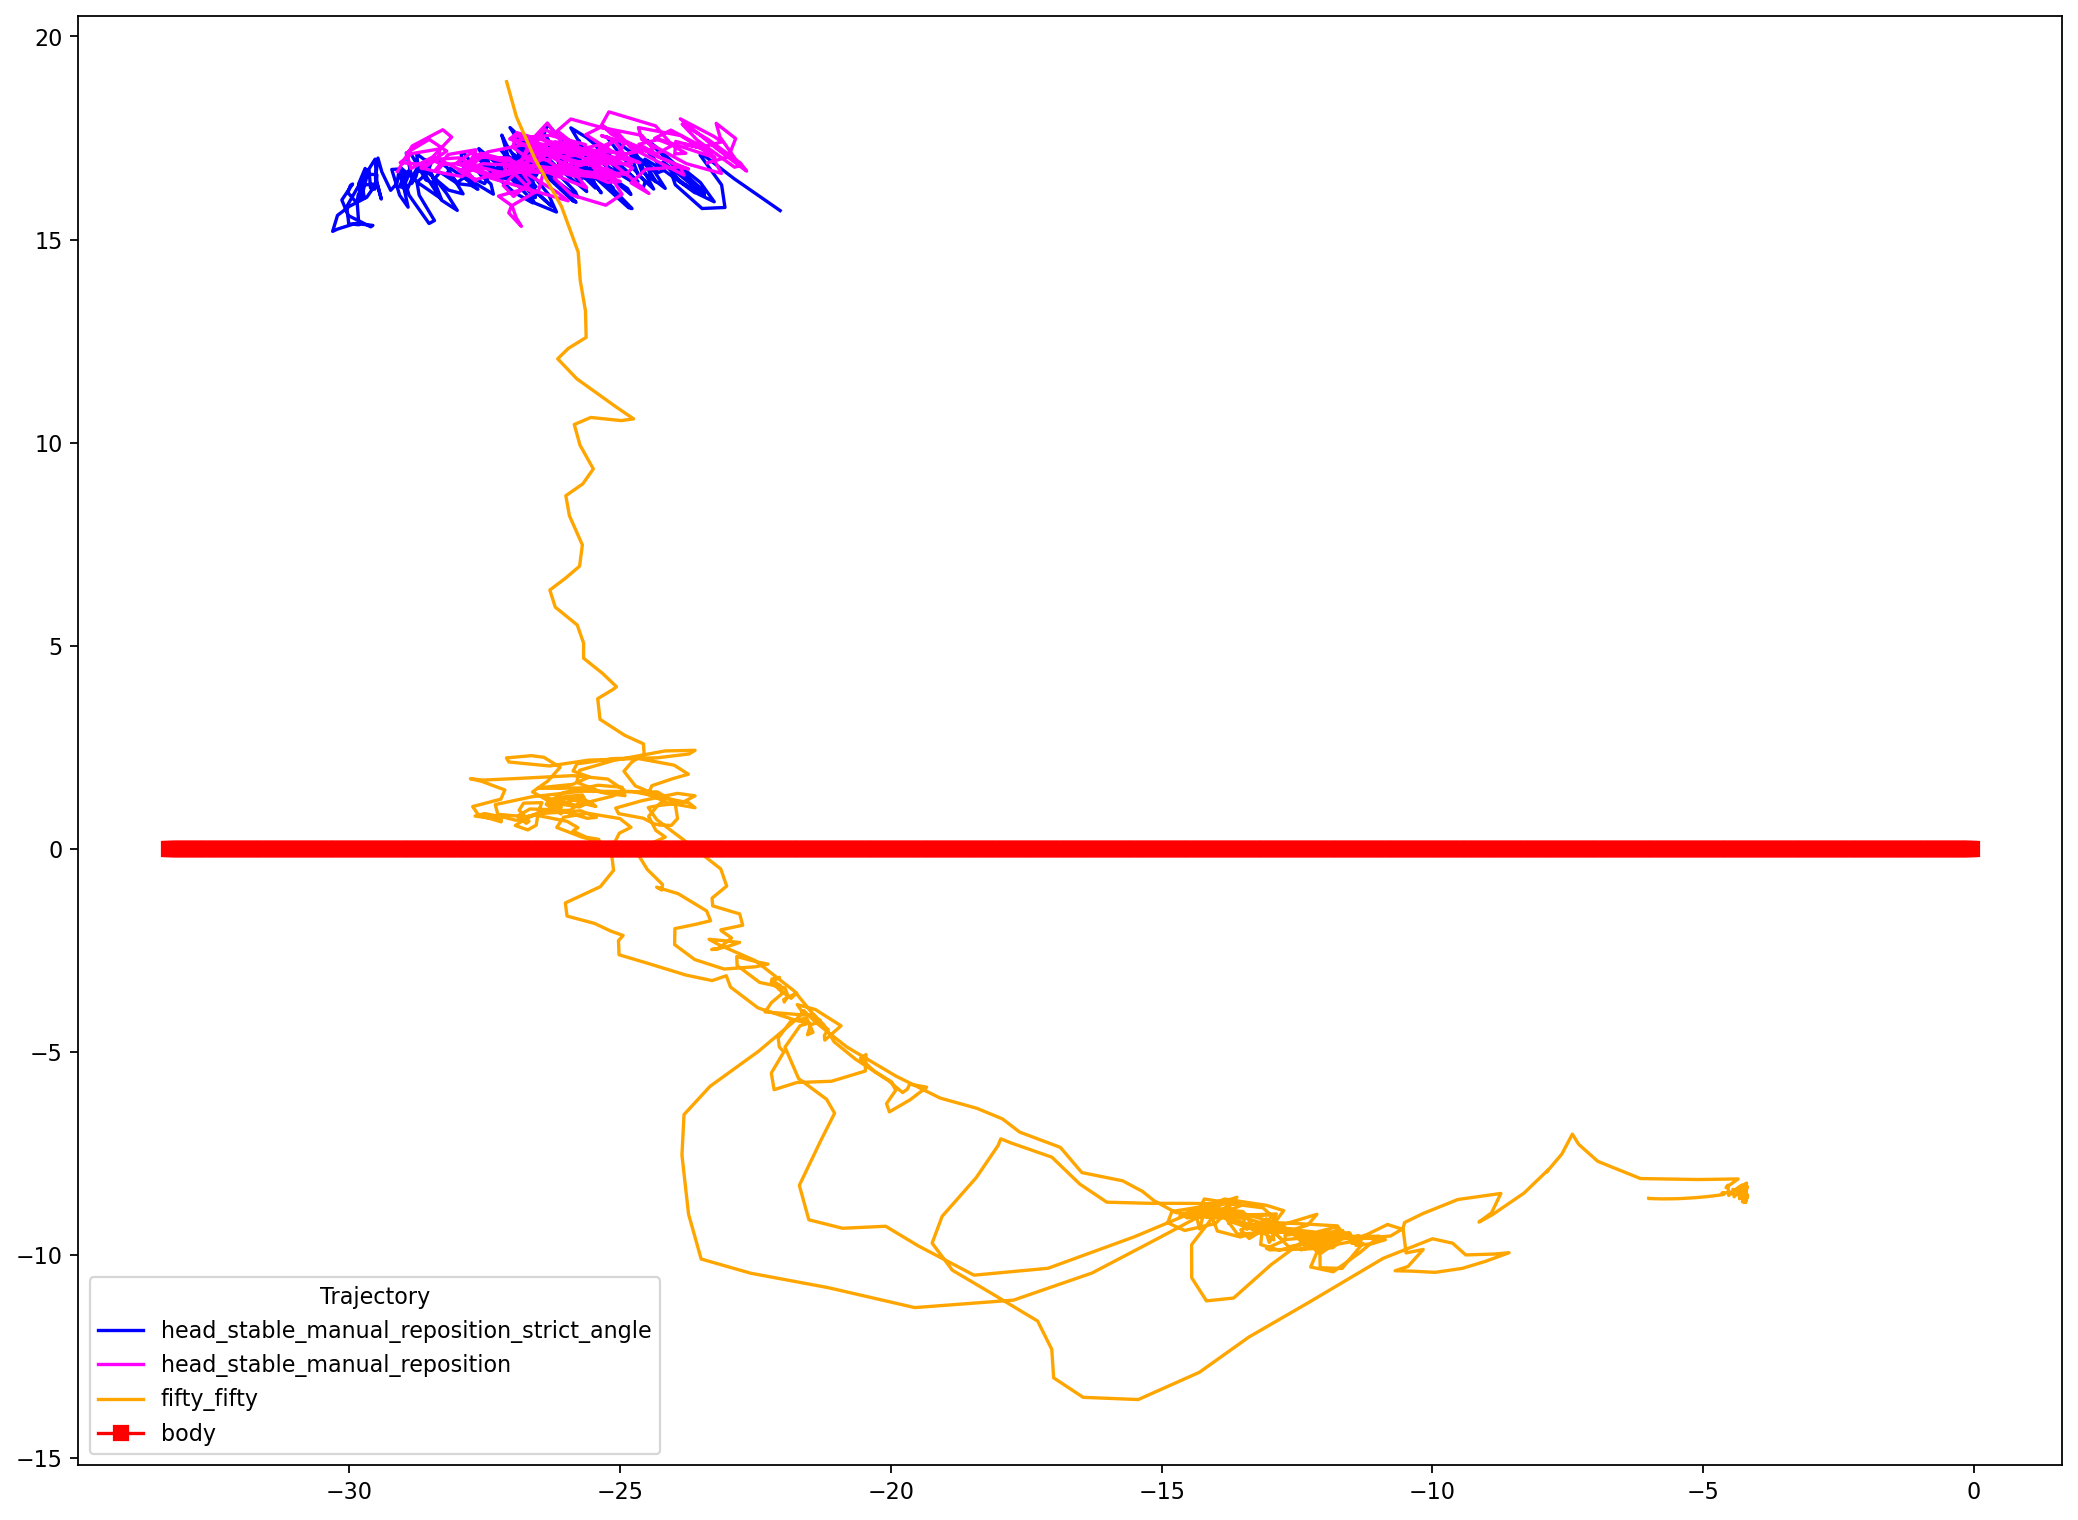
\includegraphics[width=1\textwidth]{figures/head_tracking_results/pigeon_bs_1_all_trimmed_250_550_300_550.png}
      \caption{An altered Figure \ref{fig:head_bs_1_all}, where trajectories representing $r_{head\_stable\_manual\_reposition\_strict\_angle}$ and $r_{head\_stable\_manual\_reposition}$ are trimmed to only show their head-bobbing behaviors}
      \label{fig:head_bs_1_all_trimmed}
  \end{figure}

% isolate $r_{head\_stable\_manual\_reposition}$ and $r_{fifty\_fifty}$
